\section{Ladungspumpen}
Eine Ladepumpe boostet eine Spannung hoch durch Ladungsverschiebung. Im folgenden ist $R_s$ ein Schalter-Widerstand und $T = \frac{1}{f}$ die Periode.
\begin{center}
	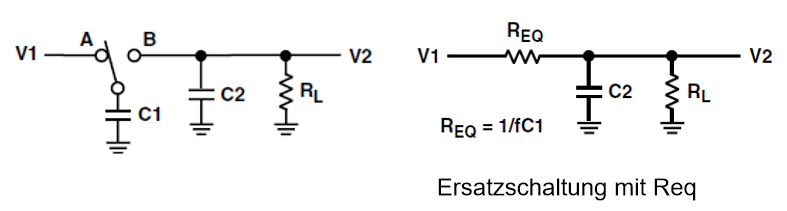
\includegraphics[width=0.8\columnwidth]{Images/ladepumpe}
\end{center}
In Phase (1) ist S1 geschlossen, in Phase (2) S2.
\begin{align}
	I_{in} = I_C = \frac{V_{in}}{R_s}\cdot e^{-\frac{t}{R_s\cdot c}} \\
	I_C = -I_{out} = -\frac{V_{in}}{R_s}\cdot e^{t - \frac{T_{per}}{2}}
\end{align}
Daraus resultiert ein durchschnittlicher Strom zur Senke von $\overline{I_{out}} = \frac{\Delta Q}{T} = \frac{C}{T} V_{in}$. Die Schalter zyklisch wieder geöffnet/geschlossen, jedes mal verteilt sich die Ladung neu auf beiden Kondensatoren bis die Ziel Spannung erreicht ist. \textbf{Hinweis}: Der Switched Capacitor hat einen äquivalenten Widerstand $R_{eq} = \frac{T}{C} = \frac{1}{f\cdot C}$ für \underline{hohe} Frequenzen
\[
V_{out} = V_{in}\cdot (1 - e^{-\frac{t}{RC}})
\]
\begin{center}
	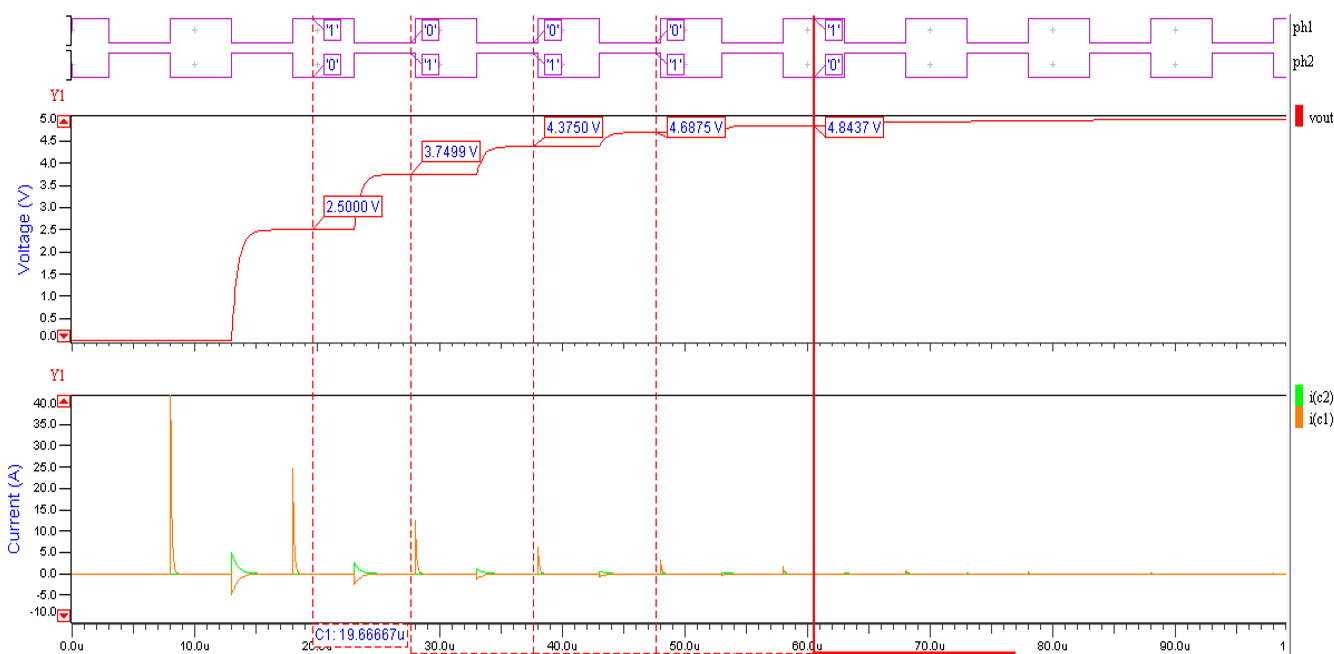
\includegraphics[width=0.6\columnwidth]{Images/ladepumpe1}
\end{center}
